\newchapter{tl2Optics}{Design of the PFF Chicane}

This is the introductory text.

\newsection{opticsIntro}{Introduction to Optics}

A basic beam line consists of focusing magnets (quadrupoles, as well as sextupoles and higher order magnets) and bending magnets (dipoles) connected by straight sections. A practical ``real world'' beam line must also include many diagnostic devices (such as beam position monitors, or BPMs) and additional elements (such as magnetic correctors) to be able to measure and remove the effects of small misalignments and imperfections in the beam line. The arrangement of devices along the line is referred to as the lattice. The collective settings (strengths) of each focusing element and the beam conditions they produce are referred to as the machine optics. The performance of the PFF system depends heavily on the lattice and optics of the correction chicane in the TL2 line (discussed in this chapter), and also in other sections at CTF3 (discussed in Chapter~\ref{c:phasePropagation}). This section presents basic aspects of lattice design and optics to introduce the terms used in the remainder of the thesis.

Each element of a beam line can be expressed as a transfer matrix \(\mathbf{R}\) that defines how it transforms the initial coordinates of a particle in the beam [REF]:
\begin{equation}
\vec{x_f} = \mathbf{R}\vec{x_0}
\end{equation}
Where \(\vec{x_0}\) and \(\vec{x_f}\) are vectors describing the initial and final state of the particle. They are six dimensional vectors and the above equation can be expanded to become:
\begin{equation}
\left( \begin{array}{c} x_f \\ x_f' \\ y_f \\ y_f' \\ t_f \\ \Delta p_f/p_0 \end{array} \right)
=
\left( \begin{array}{cccccc} 
R_{11} & R_{12} & R_{13} & R_{14} & R_{15} & R_{16}\\ 
R_{21} & R_{22} & R_{23} & R_{24}  & R_{25} & R_{26}\\ 
R_{31} & R_{32} & R_{33} & R_{34}  & R_{35} & R_{36}\\
R_{41} & R_{42} & R_{43} & R_{44}  & R_{45} & R_{46}\\
R_{51} & R_{52} & R_{53} & R_{54}  & R_{55} & R_{56}\\
R_{61} & R_{62} & R_{63} & R_{64}  & R_{65} & R_{66}\\
\end{array} \right)
\left( \begin{array}{c} x_0 \\ x_0' \\ y_0 \\ y_0' \\ t_0 \\ \Delta p_0/p_{ref} \end{array} \right)
\end{equation}
In the transverse plane the vectors \(\vec{x}\) contain the horizontal and vertical offsets (\(x\), \(y\)) and divergences (\(x' = \mathrm{d}x/\mathrm{d}s\), \(y' = \mathrm{d}y/\mathrm{d}s\), where \(s\) is the longitudinal position along the beam line). The parameters (\(x, y, s\)) define a curvilinear set of coordinates that measure the position of the particle with respect to the nominal or reference orbit, following the trajectory of the beam through bending magnets, for example [REF]. The final two longitudinal coordinates are the time offset (\(t\)) and momentum offset (\(\Delta p_0/p_{ref}\)) of the particle with respect to the reference or ideal particle. The time \(t\) is analogus to the phase of interest for the PFF system. The coefficients \(R_{ij}\) of the \(6\times6\) transfer matrix \(\mathbf{R}\) define how the final value of the \(i^{\mathrm{th}}\) coordinate after passing through the element is influenced by the initial value of the \(j^{\mathrm{th}}\) coordinate prior to the element.

The simplest and most widely used type of accelerator lattice is a FODO cell, consisting of an equally spaced focusing and defocusing quadrupole with equal strength, as shown in Figure[REF]. For small horizontal or vertical offsets from the quadrupole centre the magnetic field linearly increases with the offset [REF]. The effect of a particle travelling through a quadrupolar field is analogus to a focusing lens with a focal length \(1/kl\) where \(l\) is the length of the quadrupole and \(k\) is the strength of the quadrupole dependent on its design [REF]. Using the thin lens approximation the transfer matrix for a quadrupole is defined as [REF]:
\begin{equation}
\mathbf{R_{quad}}
=
\left( \begin{array}{cccccc} 
1 & 0 & 0 & 0 & 0 & 0\\
\pm kl & 1 & 0 & 0 & 0 & 0 \\
0 & 0 & 1 & 0 & 0 & 0 \\
0 & 0 & \mp kl & 1 & 0 & 0 \\
0 & 0 & 0 & 0 & 1 & 0 \\
0 & 0 & 0 & 0 & 0 & 1 \\
\end{array} \right)
\end{equation}
The final horizontal divergences of a particle after traversing a quadrupole, using the above matrix, are \(x_f' = x_i' \pm klx_i\) and \(y_f' = y_i' \mp kly_i\). A quadrupole that focuses the beam in one plane therefore defocuses the beam in the other transverse plane. In a FODO cell a horizontally focusing quadrupole and horizontally defocusing quadrupole are used together to give a net focusing effect in both planes [REF]. The complete effect of a FODO cell on a particle can be determined by multiplying the transfer matrices of each element:
\begin{equation}
\mathbf{R_{FODO}} = \mathbf{R_{F} \times R_{drift} \times R_{D}}
\end{equation}
\begin{equation}
\vec{x_f} = \mathbf{R_{FODO}}\vec{x_0}
\end{equation}
Where \(R_{F}\) and \(R_{D}\) are the transfer matrices of the focusing and defocusing quadrupoles respectively and \(R_{drift}\) is the transfer matrix for the drift space between the quadrupoles. 

The same approach can be used to construct the transfer matrix for any complete beam line, and several of the transfer matrix coefficients are of particular interest for the PFF system both in the TL2 and TL1 transfer lines at CTF3. These will be explained in more detail later in this chapter but include mostly the coefficients related to horizontally deflecting (or ``kicking'') the beam, so the \(R_{2j}\) and \(R_{i2}\) terms including the horizontal divergence, and the coefficients related to the final beam phase, so the \(R_{5j}\) terms. At CTF3 optics and transfer matrices are calculated using a MADX model of the machine [REF]. MADX is one of the leading tools avilable for the design and simulation of particle accelerators [REF]. All the optics terms presented in this thesis use MADX coordinates and units [REF]. In some cases these are slightly modified from the coordinates defined above, and these differences are explained later when relevant.

The previous discussion shows how the propagation of a single particle through a beam line can be modelled. The matrix formalism above can be adjusted to describe the trajectories of many particles by replacing the column vectors \(\vec{x}\) with matrices of many column vectors describing each particle. However, to understand the properties of a complete beam it is also useful to introduce the general solution to the tranverse equations of motion (Hill's Equation) [REF]:
\begin{equation}
x_i(s) = \sqrt{\beta_x(s)\epsilon_x}\cos[\mu_x(s) + \delta_{xi}]
\end{equation}
Replacing \(x\) with \(y\) gives the equivalent solution in the vertical plane. The subscript \(i\) refers to the \(i^\mathrm{th}\) particle. The transverse motion follows a modified harmonic oscillation with amplitude \(\sqrt{\beta_x(s)\epsilon_x}\). The betatron (or beta) function \(\beta_x(s)\) varies along the beam line and depends on the lattice and optics, whilst the beam emittance \(\epsilon_x\) is a preserved quantity [REF]. The phase advance \(\mu_x(s)\) defines the phase of the oscillation at each point along the lattice, with each particle having an initial phase offset \(\delta_{xi}\).

The solution has a constant of motion known as the Courant-Snyder invariant [REF]:
\begin{equation}
\gamma_x x^2 + 2\alpha_x x x' + \beta_x x'^2 = \epsilon_x 
\end{equation}
Where the explicit dependence on \(s\) of all the parameters apart from the emittance has been dropped for readability. \(\beta_{x}\), \(\alpha_{x}\) and \(\gamma_{x}\) are collectively known as the Twiss parameters [REF], where the \(\alpha_x\) and \(\gamma_x\) functions relate to the beta function as follows [REF]:
\begin{align}
\alpha_x &= -\frac{1}{2}\frac{\mathrm{d}\beta_x}{\mathrm{d}s} \\
\gamma_x &= \frac{1+\alpha_x^2}{\beta_x}
\end{align}
The Courant-Snyder invariant defines an ellipse with area \(\pi\epsilon_x\) in \((x, x')\) phase space. All particles therefore follow elliptical trajectories in phase space as they progress through the beam line. At any point along the lattice one standard deviation of particles in a gaussian beam are contained within an envelope of \(x(s) \leq \sqrt{\beta_x(s)\epsilon_x}\) [REF]. The beta function therefore defines the beam size at any point in the lattice (considering only transverse first order effects). In a FODO cell, for example, the optics is such that the beta function is minimum at the centre of the defocusing quadrupole and maximum at the centre of the focusing quadrupole [REF].

[TODO: fodo/ellipse figures? Or just text ok?]

\newsection{kickers}{Kicker Design}

The two electromagnetic kickers provide the phase correction in the PFF system by deflecting the beam on to longer or shorter paths in the TL2 chicane. They have been designed and built by INFN, Italy [REF], based on a similar design used at the DA\(\mathrm{\Phi}\)NE collider [REF]. A schematic of the kicker design is shown in Figure~\ref{f:kickerSchematic}. It consists of two parallel conducting strips placed along the left and right side of the beam pipe. Each strip is approximately one metre in length and the horizontal separation between the strips is 40~mm. The strips are tapered at their ends to reduce coupling impedance (to reduce the voltage induced on the strips by the beam) [REF].

At each end of each strip there is a transition to a 50~\(\mathrm{\Omega}\) HN-type connector. A voltage is applied to the downstream end of each kicker strip, with opposite polarity on each side, for example \(+V\) to the left strip and \(-V\) to the right strip. The voltage is produced by the amplifier discussed in Section~\ref{s:amplifierSetup}, and the voltage leaving the upstream ends of the kicker strips is also terminated back at the amplifier. The applied voltage \(V(t)\) creates a horizontal, position independent, electric field and vertical magnetic field between the strips with related amplitudes as follows [REF]:
\begin{eqnarray}
E_x &\sim& V(t) \\
B_y &\sim& \frac{V(t)}{c}
\end{eqnarray}
Where \(c\) is the speed of light. By the Lorentz force an electron in the beam propagating with speed \(v\) from the upstream end of the kicker to the downstream end (in the opposite direction to the voltage applied to the strips) experiences the following horizontal force [REF]:
\begin{equation}
F_x = e(E_x + vB_y) \sim e(1+\beta)V(t) \sim 2eV(t)
\end{equation}
Where \(e\) is the charge of an electron and \(\beta = v/c\). The final expression holds for an ultra-relativistic particle where \(\beta \simeq 1\), which is true for the CTF3 beam. In this case the forces resulting from the electric and magnetic fields have the same magnitude and direction. If the voltage were applied to the upstream end of the strip rather than the downstream end, the magnetic field would be in the opposite direction and the resulting electric and magnetic forces would cancel. 

With the voltage correctly applied to the downstream end of the strips the force is as above and the kicker imparts a horizontal deflection to the beam. The kicker design gives a horizontal deflection of 1~mrad for an applied voltage of \(\pm1.26~kV\) to each strip [REF], assuming the CTF3 beam energy of around 135 MeV [REF]. This value together with the peak voltage output from the amplifier and the optics of the TL2 chicane (as described below) defines the maximum phase offset that can bwe corrected by the PFF system (Section~\ref{ss:corrRange}).

\begin{figure}
  \centering
  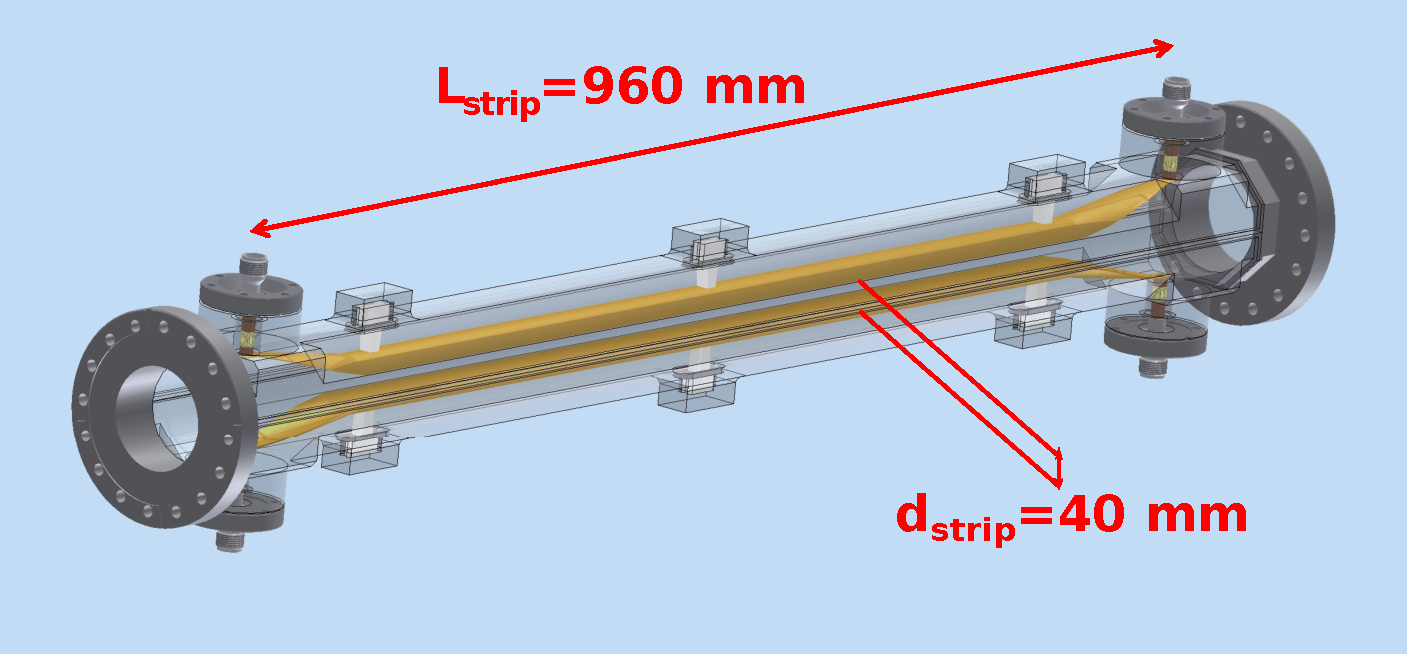
\includegraphics[width=0.8\textwidth]{Figures/optics/kickerSchematic}
  \caption{Technical drawing of the kicker design. The kicker is shown in a vertical orientation with the strips on the top and bottom. When installed in the beam line the kicker is oriented with the strips on the left and right, in order to create a horizontal electric field between the strips.}
  \label{f:kickerSchematic}
\end{figure}

\newsection{tl2}{TL2}

The transfer line TL2 at CTF3 transports the beam from the exit of the combiner ring to the experimental area CLEX (see Figure~\ref{f:ctfLayout}). The whole line is approximately 35~m long and contains both vertical and horizontal chicanes to align the outgoing combiner ring beam line to the CLEX entrance. The PFF system attempts to correct the beam phase using the horizontal chicane at the end of TL2, where the two kickers are installed. Further details of the design of TL2 can be found in [REF].

The diagram in Figure~\ref{f:newTL2Lattice} shows a birds-eye view of the TL2 line and the lattice of the line. To interpret the diagram it is useful to introduce the device naming convention at CTF3. Devices have names of the form:
\begin{center}
[CC].[QF][D][0840]
\end{center}
The first two letters refer to the section of the machine, with the prefix CC used for TL2. These are not included in the diagram to improve readability. In Chapters~\ref{c:phaseMons}~and~\ref{c:phasePropagation} the prefix CT is used to refer to the CT-line after the linac and transfer line TL1 prior to the combiner ring. The second group of letters refer to the type of device, the main ones being QF and QD for horizontally focusing and defocusing quadrupoles, BH and BV for horizontal and vertical dipoles, BP for beam position monitors (BPMs) and DH and DV for horizontal and vertical corrector magnets. The last letter indicates the type of that device, with four different designs of quadrupole used along the TL2 line (G-type, H-type, L-type and D-type), for example. The four final numbers indicate the position of that device along the line, in ascending order from the beginning to the end of the line.

The horizontal chicane of interest for the PFF system starts at the dipole CC.BHG0500 and ends at the dipole CC.BHG0800. The first (500) and last (800) dipoles bend the beam through \(+31^\circ\) and \(-31^\circ\) respectively. Inside the chicane there are two further dipoles of a different type -- CC.BHH0600 and CC.BHH0700, which deflect the beam through \(+17^\circ\) and \(-17^\circ\) respectively. Some details on the differences between the two types of dipole are given in Section~\ref{ss:modelErrorSources}. The resulting overall chicane has a ``dog leg'' shape around 12~m in length, with three straight sections around 4~m in length between the bending magnets. Each straight section contains a triplet of quadrupoles and either one (in the first and last sections) or two (in the middle section) BPMs (of the BPI type [REF]). Although the quadrupoles are labelled as horizontally focusing or defocusing the polarity of the current sent to each can be reversed so that it focuses in the opposite plane. The F or D labels refer to whether the magnet is horizontally focusing or defocusing when a positive current is sent to the quadrupole.

Other features along the TL2 line that are important for the derivation of optics seen later in this chapter include the vertical chicane and two long drift spaces without focusing elements. The vertical chicane starts and ends at CC.BVA0300 and CC.BVB0400 respecitvely, and contains a triplet of quadrupoles. Between the quadrupole CC.QFD0840 (the last shown in the diagram) and CC.QFL0910, there is a long drift space of around 4~m with no focusing elements as the beam pipe passes through in to the neighbouring building where the CLEX area is located. Between the quadrupole CC.QFH0230 and CC.QFL0270 there is another long drift space, around 7~m. The Twiss beta and alpha functions entering these long drifts must be carefully chosen to avoid unrecoverable growth in the beam size.

[TODO: picture of TL2/chicane]

\begin{landscape}
\begin{figure}
  \centering
  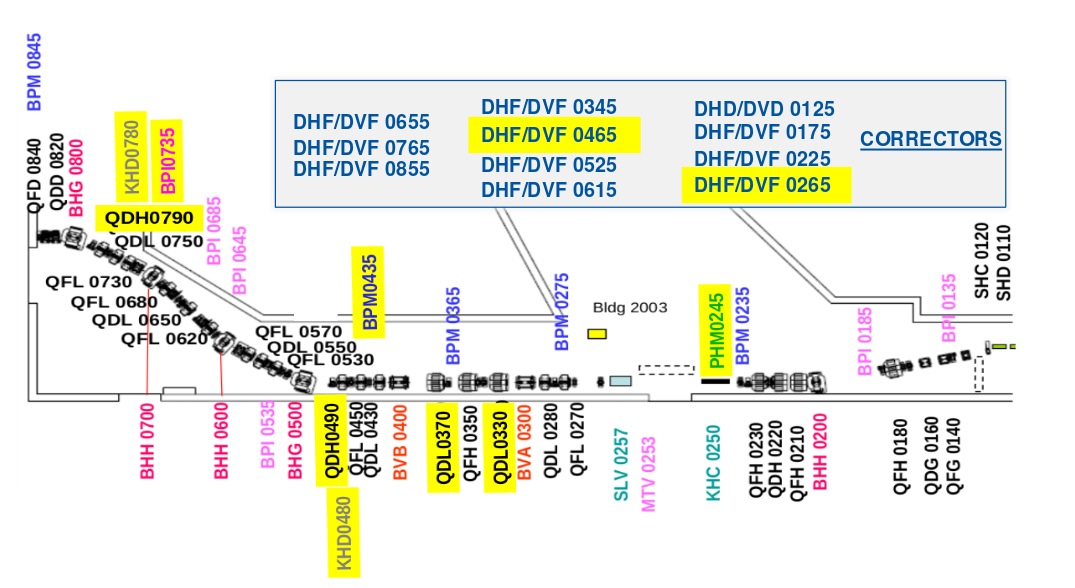
\includegraphics[width=\hsize]{Figures/optics/newTL2Lattice}
  \caption{New TL2 lattice for PFF. Changes highlighted yellow.}
  \label{f:newTL2Lattice}
\end{figure}
\end{landscape}

\subsection{Integration of PFF Hardware}
\label{ss:tl2PFFIntegration}

Due to building and cost constraints the PFF prototype had to make use of the pre-existing layout of the TL2 horizontal chicane, with only minor modifications possible to accommodate the PFF hardware. These changes are highlighted in yellow in Figure~\ref{f:newTL2Lattice}.

As the chicane was already densely packed with quadrupoles and other devices the integration of the two kickers was not straightforward. To maintain the functionality of the lattice quadrupoles could not be removed, and thus instead the kickers have been installed inside wide aperture `H-type' quadrupoles [REF]. Two `L-type' quadrupoles (now CC.QDL0330 and CC.QDL0370) from the horizontal chicane were swapped with two `H-type' quadrupoles (now CC.QDH0490 and CC.QDH0790) from the vertical chicane. The two PFF kickers, CC.KHD0480 and CC.KHD0780, are then installed inside the aperture of these quadrupoles, prior to the first and last dipole of the horizontal chicane. In addition, two magnetic correctors (now CC.DHF0465 and CC.DHF0765) were installed around the PFF kickers to facilitate a complementary, large range but low bandwidth, slow phase correction [REF]. A schematic of the installation of one of the kickers inside the quadrupole and corrector is shown in Figure~[REF]. The kicker CC.KHD0480 will also be referred to as the first kicker (or K1), and CC.KHD0780 as the second kicker (or K2).

Apart from the quadrupoles and correctors two BPMs (now CC.BPI0435 and CC.BPI0735) had to be moved slightly to vacate the area now occupied by the kickers. Finally, a slot near the start of TL2 (CC.PHM0245) was reserved for the installation of an additional phase monitor to verify the beam phase prior to the correction. Eventually this was not necessary and has not been pursued as the 2~cm aperture of the phase monitors (Section~\ref{s:phaseMonDesign}) compared to the 4~cm aperture of the neighbouring beam pipe would have created beam setup difficulties for normal operation at CTF3 [REF].

[TODO: pictures/diagram of kickers in quadrupole]

\newsection{tl2OpticsReqs}{TL2 Optics Constraints}

To take in to account the changes made to the TL2 lattice new optics were needed. This section summarises the various optics constraints that must be met in TL2. These can be split in to two types -- the nominal optics constraints, required to recover the same (or similar) beam conditions as before the changes, and the new optics constraints for operation of the PFF system, required to create the desired phase shifting behaviour in the chicane.

\subsection{Nominal Optics Constraints}
\label{ss:nominalOpticsReqs}



\subsubsection{Dispersion}

The trajectory of a particle through a dipole depends on its energy, with lower energy particles following a smaller radius of curvature and high energy particles a larger radius. After a dipole the orbit of a particle though the following elements therefore depends on its energy. This effect is characterised using the horizontal and vertical dispersion, \(D_x\) and \(D_y\), which are defined as follows (considering only the energy component of the beam orbit):
\begin{eqnarray}
x(s) &=& D_x(s)\left(\frac{\Delta p}{p}\right) \\
y(s) &=& D_y(s)\left(\frac{\Delta p}{p}\right)
\end{eqnarray}
The dispersions \(D_x(s)\) and \(D_y(s)\) vary along the lattice and are equivalent to the transfer matrix coefficients \(R_{16} = D_x\) and \(R_{36} = D_y\). 

Optics are usually created so that there is no dispersion (\(D_{x} = D_{y} = 0\)) in straight sections. However, inside chicanes and rings the dispersion can never always be zero. To give zero dispersion in the straight sections the dispersion must therefore be closed at the exit of all bending sections. Dispersion closure means that both the dispersion and its derivative (\(D_x' = \mathrm{d}D_x/\mathrm{d}s\), and \(D_y' = \mathrm{d}D_y/\mathrm{d}s\)) are zero at the exit from the chicane or ring. In TL2 this condition applies after the bend CC.BHH0200 at the start of the line and at the exit of the horizontal chicane (CC.BHG0800) for the horizontal dispersion, and at the exit of the vertical chicane (CC.BVB0400) for the vertical dispersion.

Within the bending sections the magnitude of the dispersion should be kept as small as possible whilst meeting the other optics constraints. At CTF3 there can be peak-to-peak energy offsets at around the \(\pm1\%\) level [REF]. Dispersion is then usually the largest contribution to the beam size, with a dispersion of 1~m giving excursions up to \(\pm1\)~cm in individual particle orbits, for example. The diameter of the beam pipe in bending sections at CTF3 is 10~cm in most cases, as opposed to 4~cm in straight sections, in order to minimise the effects of dispersion dependent beam size growth on the beam transport [REF]. However, the second kicker installed in the chicane for the PFF system (CC.KHD0780) only has the normal 4~cm aperture (2~cm radius).  Dispersion around the second kicker must therefore be kept well below 2~m to avoid losing a fraction of off-energy particles on the kicker strips.

\subsubsection{Twiss Functions}
beta functions

matching from CR and in to CLEX

long drifts

Normalised emittance around 150 micrometres (best case?)
Gamma is 135 MeV/0.5 MeV = 270 at CTF3
Normalised emittance is beta*gamma*emittance
real emittance is 0.5555 micrometres
50~m beta function gives around +/- 0.5 cm beam size

\begin{table}
  \begin{center}
    \begin{tabular}{|c c|}
	   \hline
       Parameter & Value \\
       \hline
       \(\beta_x\) & 7.26~m\\
	   \(\beta_y\) & 5.90~m\\
	   \(\alpha_x\) & -4.84\\
	   \(\alpha_y\) & -1.27\\
	   \hline
    \end{tabular}
    \caption{Initial twiss parameters for the TL2 line, taken at the entrance to CC.QFH0210.}
  	\label{t:tl2InitTwiss}
  \end{center}
\end{table}

\subsubsection{R56}

The dispersion describes how the transverse orbit of a particle is changed by its energy in bending sections as already discussed. These differences can also change the longitudinal path length of the particle's trajectory, thereby shifting the particle's phase (described by the time \(t\), the fifth coordinate in the matrix formalism). This effect is described by the transfer matrix coefficient \(R_{56}\):
\begin{equation}
t_{f} = t_{i} + R_{56}\left(\frac{\Delta p}{p}\right)
\end{equation}

The \(R_{56}\) value between the entrance and exit of all bending sections at CTF3 is nominally zero so that there is no transformation of energy jitter in to phase jitter. In TL2 this places the constraints for \(R_{56}\) to be zero between the entrance and exit of the vertical chicane (CC.BVA0300 to CC.BVB0400) and between the entrance and exit of the horizontal chicane (CC.BHG0500 to CC.BHG0800).

\subsection{PFF Optics Constraints}
\label{ss:pffOpticsReqs}

All the additional PFF optics constraints place requirements on the transfer matrix coefficients between the two kickers, from the exit of the first kicker to the entrance of the second kicker. There are two sets of constraints, one to maximise the correction range of the PFF system and the other to ensure the PFF system does not degrade the orbit stability of the beam after the chicane.

\subsubsection{Correction Range}

The PFF system clearly requires the path length between the two kickers to depend on the applied kick. This difference in path length dependent on the voltage applied to the kickers is what shifts the time or phase of the beam to form the correction. The transfer matrix coefficient that relates the time variable to the deflection induced by the kickers is \(R_{52}\):
\begin{equation}
t_{K2} = t_{K1} + R_{52}x_{K1}'
\end{equation}
Where \(t_{K1}\) and \(t_{K2}\) are the time offset of the particle at the exit of the first kicker and at the entrance to the second kicker respectively. \(x_{K1}\) is the divergence at the exit of the first kicker resulting from the applied kick. MADX uses units of metres for its `time' variable [REF]. To convert these distances in to 12~GHz degrees they must be multiplied by the constant factor \(360/\lambda_{\mathrm{12GHz}}\), where \(\lambda_{\mathrm{12GHz}} = 2.5\)~cm is the 12~GHz wavelength. Directly in terms of phase (in degrees) the equation above therefore becomes:
\begin{equation}
\phi_{K2} = \phi_{K1} + R_{52}\left(\frac{360}{\lambda_{\mathrm{12GHz}}}\right)x_{K1}'
\end{equation}
Where \(\phi_{K2}\) is the phase at the entrance to the second kicker (the corrected phase) and \(\phi_{K1}\) is the initial uncorrected phase at the exit of the first kicker. The maximum value of \(x_{K1}'\) is fixed by the peak voltage output from the kicker amplifiers and the design of the kickers themselves. To obtain the largest possible correction range for the PFF system given the parameters of the hardware, the \(R_{52}\) transfer matrix coefficient should be as large as possible. For example, with \(R_{52} = 1\)~m and a maximal kick of \(x_{K1}' = \pm 1\)~mrad, the correction range of the PFF system would be \(\pm 14.4\)~degrees.

The path length difference in the chicane largely results from differing trajectories in the dipoles. In this way it is somewhat analogus to the dispersion, which describes the energy dependent difference in beam orbit after dipoles. This has the unfortunate consequence of leading to optics with high \(R_{52}\) values also tending to have high peak dispersion values in the chicane. The PFF optics must therefore be a compromise that achieves a reasonable correction range whilst keeping the dispersion small enough to avoid beam losses in the chicane.

\subsubsection{Orbit Closure}

The PFF system should not change the beam orbit after the chicane, which means the beam position and divergence after the second kicker must be independent of the applied kicks. In other words, the second kicker must close the horizontal orbit bump created by the first kicker. To understand the further constraints this places on the optics the position, \(x_{K2}\), and divergence \(x_{K2}'\) of the beam at the entrance to the second kicker will be considered first. These can be expressed as:
\begin{eqnarray}
x_{K2} &=& R_{11}x_{K1} + R_{12}x_{K1}' \\
x_{K2}' &=& R_{21}x_{K1} + R_{22}x_{K1}'
\end{eqnarray}
Where \(x_{K1}\) and \(x_{K1}'\) are the position and divergence at the exit of the first kicker, and \(R_{11}\), \(R_{12}\), \(R_{21}\) and \(R_{22}\) are transfer matrix coefficients for the optics between the exit of the first kicker and the entrance to the second kicker. The beam position at the exit of the first kicker is proportional to the applied kick:
\begin{equation}
x_{K1} = m x_{K1}'
\end{equation}
Here \(m\) is a constant that depends on the properties of the kicker and also on the strength of the quadrupole CC.QDH0490 within which the kicker is installed (Section~\ref{ss:tl2PFFIntegration}). Substituting this expression in to the equations for \(x_{K2}\) and \(x_{K2}'\) gives:
\begin{eqnarray}
x_{K2} &=& \left(R_{11} + \frac{R_{12}}{m}\right)x_{K1} \\
x_{K2}' &=& (m R_{21} + R_{22})x_{K1}'
\end{eqnarray}
As stated \(x_{K2}\) and \(x_{K2}'\) are defined above at the entrance to the second kicker. The requirement for the PFF chicane optics is that the position and divergence at the exit of the second kicker are zero independent of the applied kicks. However, a derivation of the exact expression for the optics requirements between the kickers in order to close the orbit at the exit of the second kicker is complicated by the fact that the quadrupole around the second kicker, CC.QDH0790, can have a different strength to the quadrupole around the first kicker. 

For the purpose of the discussion here the simplified case where CC.QDH0790 has the same strength but opposite polarity (focuses in the opposite plane) as CC.QDH0490 will be considered. The ideal case where the two kickers can be powered with the same magnitude voltage but opposite polarity is also assumed. With these conditions, the second quadrupole/kicker effectively have precisely the opposite effect on the beam as the first quadrupole/kicker. To close the orbit after the second kicker the position and divergence at the entrance to the second kicker must therefore meet the following criteria:
\begin{eqnarray}
x_{K2} &=& -x_{K1} \\
x_{K2}' &=& x_{K1}'
\end{eqnarray}
Comparing these two expressions to the previously derived equations for \(x_{K2}\) and \(x_{K2}'\) then yields the following optics constraints:
\begin{eqnarray}
R_{11} + \frac{R_{12}}{m} &=& -1  \label{e:orbClosConst1} \\
m R_{21} + R_{22} &=& +1 \label{e:orbClosConst2}
\end{eqnarray}
There are many possible solutions to these expressions, with the simplest example being \(R_{11} = -1\), \(R_{12} = 0\), \(R_{21} = 0\) and \(R_{22} = 1\). However, the optics matching (Section~\ref{s:matchedOptics}) allows the quadrupoles CC.QDH0490 and CC.QDH0790 to have different strengths. MADX is then used to model the actual beam orbit in the chicane and the figure of merit is for the simulated orbit to be closed after the second kicker, rather than for the above constraints to be met. Nevertheless, the optics eventually created do satisfy Equations~\ref{e:orbClosConst1}~and~\ref{e:orbClosConst2} within several percent [REF].

%First assuming a simplified case of zero length kickers (with only the divergence changing in the kicker and not the beam position), the position \(x_{K2}\), and divergence, \(x_{K2}'\), of the beam at the entrance to the second kicker can be expressed as:
%\begin{eqnarray}
%x_{K2} &=& R_{12} x_{K1}' \\
%x_{K2}' &=& R_{22} x_{K1}'
%\end{eqnarray}
%Where \(x_{K1}\) and \(x_{K1}'\) are the position and divergence at the exit of the first kicker, and \(R_{12}\) and \(R_{22}\) are transfer matrix coefficients for the optics between the exit of the first kicker and the entrance to the second kicker. The position and divergence after the second kicker, \(x_f\) and \(x_f'\) are then given by:
%\begin{eqnarray}
%x_{f} &=& x_{K2} \\
%x_{f}' &=& x_{K2}' \mp x_{K1}'
%\end{eqnarray}
%The equation for the divergence assumes the ideal case where both kickers are powered with the same magnitude voltage. Inserting the expressions for \(x_{K2}\) and \(x_{K2}'\) above places the optics requirements \(R_{12} = 0\) and \(R_{22} = \pm 1\) to ensure orbit closure after the second kicker.

\newsection{opticsMeas}{TL2 Optics Measurements}

\subsection{Method}
\label{ss:opticsMethod}

change all correctors along line in h and v

compare measured orbit in bpms to expectation from madx model

\subsection{Results}
\label{ss:opticsResults}

plots from near start tl2 in H and V showing large discrepancy

\subsection{Sources of Errors in MADX Model}
\label{ss:modelErrorSources}

\subsubsection{Dipole Edge Focusing}
\label{sss:edgeFocusing}

theory of edge focusing with different types of dipole

\subsubsection{Quadrupole Strengths}
\label{sss:quadStrengths}

not measured/error for one type

\subsection{Corrections to MADX Model}
\label{ss:modelCorrections}

plot of effect of adjusting edge focusing

plot of effect of adjusting quad strengths

statistics, sum sq diff in bpms?

something about the process? mixture of by hand/matching

\begin{figure}
  \centering
  
\includegraphics[width=0.8\textwidth]{Figures/optics/opticsCorrVsOrig}
  \caption{Mean phase along.}
  \label{f:opticsCorrVsOrig}
\end{figure}

\newsection{matchedOptics}{Matched TL2 Optics}

\subsection{Nominal Optics}
\label{ss:nominalMatched}

maybe not needed? but nice to compare to pff. plots of dx, betas, r56

\subsection{PFF Optics}
\label{ss:pffMatched}

something about the process? different sets of optics with larger dispersion etc.?

final result

\begin{table}
  \begin{center}
    \begin{tabular}{|c c|}
	    \hline
        Quadrupole & Current \\ \hline
		CC.IQFH0210 &	47.00~A \\
		CC.IQDH0220 &	48.83~A \\
		CC.IQFH0230 &	31.75~A \\
		CC.IQFL0270 &	14.44~A \\
		CC.IQDL0280 &	24.96~A \\
		CC.IQDL0330 &	24.57~A \\
		CC.IQFH0350 &	40.07~A \\
		CC.IQDL0370 &	24.57~A \\
		CC.IQDL0430 &	0.16~A \\
		CC.IQFL0450 &	0.17~A \\
		CC.IQDH0490 &	-6.05~A \\
		CC.IQFL0530 &	21.94~A \\
		CC.IQDL0550 &	27.57~A \\
		CC.IQFL0570 &	30.19~A \\
		CC.IQFL0620 &	-1.16~A \\
		CC.IQDL0650 &	-10.46~A \\
		CC.IQFL0680 &	-5.96~A \\
		CC.IQFL0730 &	-7.77~A \\
		CC.IQDL0750 &	-14.81~A \\
		CC.IQDH0790 &	6.32~A \\
		CC.IQDD0820 &	63.49~A \\
		CC.IQFD0840 &	76.53~A \\
		CC.IQFL0910 &	-11.97~A \\
		CC.IQDL0920 &	-12.84~A \\
	   \hline
    \end{tabular}
    \caption{Quadrupole power supply currents to set in the new PFF TL2 optics for a beam energy of 135~MeV.}
  	\label{t:pffOpticsQuads}
  \end{center}
\end{table}

\begin{table}
  \begin{center}
    \begin{tabular}{|c c c|}
	   \hline
       Parameter & Constraint & Value \\ \hline
       \(\beta_x\) & (Max \(<100\)~m) & 55.3~m at CC.QFL0270\\
	   \(\beta_y\) & (Max \(<100\)~m) & 72.1~m at CC.QDL0330\\
	   \(|\alpha_x|\) & (Max \(<30\)) & 43.3 at CC.QFL0270\\
	   \(|\alpha_y|\) & (Max \(<30\)) & 75.9 at CC.QFL0330\\
	   \(|D_x|\) & Max \(<2.5\)~m & 1.16~m at CC.QDL0650\\
	   \(|D_y|\) & Max \(<1\)~m & 0.11~m at CC.QDL0330\\
	   \(|D_x|\) & \(\ll 2\)~m at K2 & 0.98~m\\
	   \(D_x\) & 0~m at CC.BHG0800 & \(9\times10^{-7}\)~m\\
	   \(D_x'\) & 0 at CC.BHG0800 & \(-6\times10^{-6}\)\\
	   \(D_y\) & 0~m at CC.BVB0400 & \(4\times10^{-5}\)~m\\
	   \(D_y'\) & 0 at CC.BVB0400 & \(-6\times10^{-5}\)\\
	   \(|R_{52}|\) & \(\gg 0\)~m from K1 to K2 & 0.74~m\\
	   \(x\) & 0~m after K2 & \(3\times10^{-7}\)~m (1~mrad kick)\\
	   \(x'\) & 0 after K2 & \(-5\times10^{-7}\) (1~mrad kick)\\
	   \(R_{56}\) & 0~m from CC.BHG0500 to CC.BHG0800 & -0.18~m\\
	   \hline
    \end{tabular}
    \caption{Summary of constraints and their matched values in the new TL2 PFF optics.}
  	\label{t:pffOpticsVals}
  \end{center}
\end{table}


\begin{landscape}
\begin{figure}
  \centering
  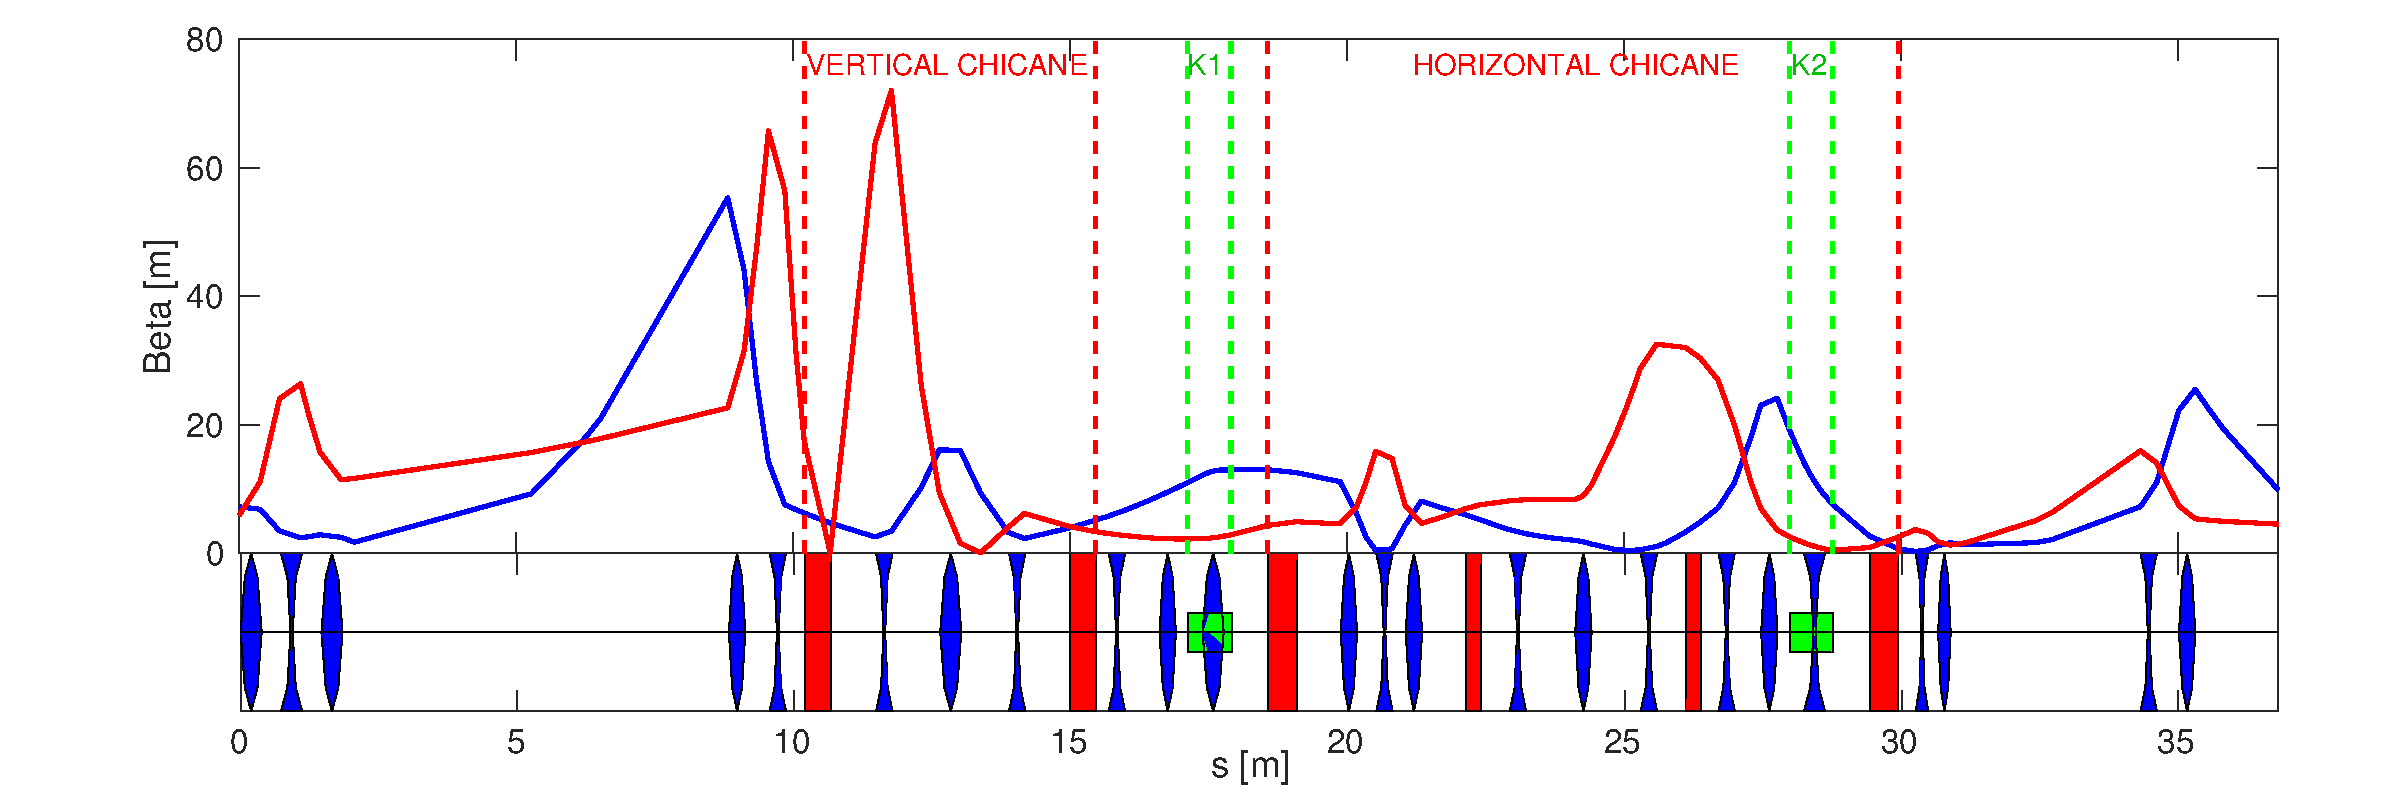
\includegraphics[width=0.85\hsize]{Figures/optics/pffOpticsBeta}
  \caption{Horizontal and vertical beta functions in the new TL2 optics.}
  \label{f:pffOpticsBeta}
  \centering
  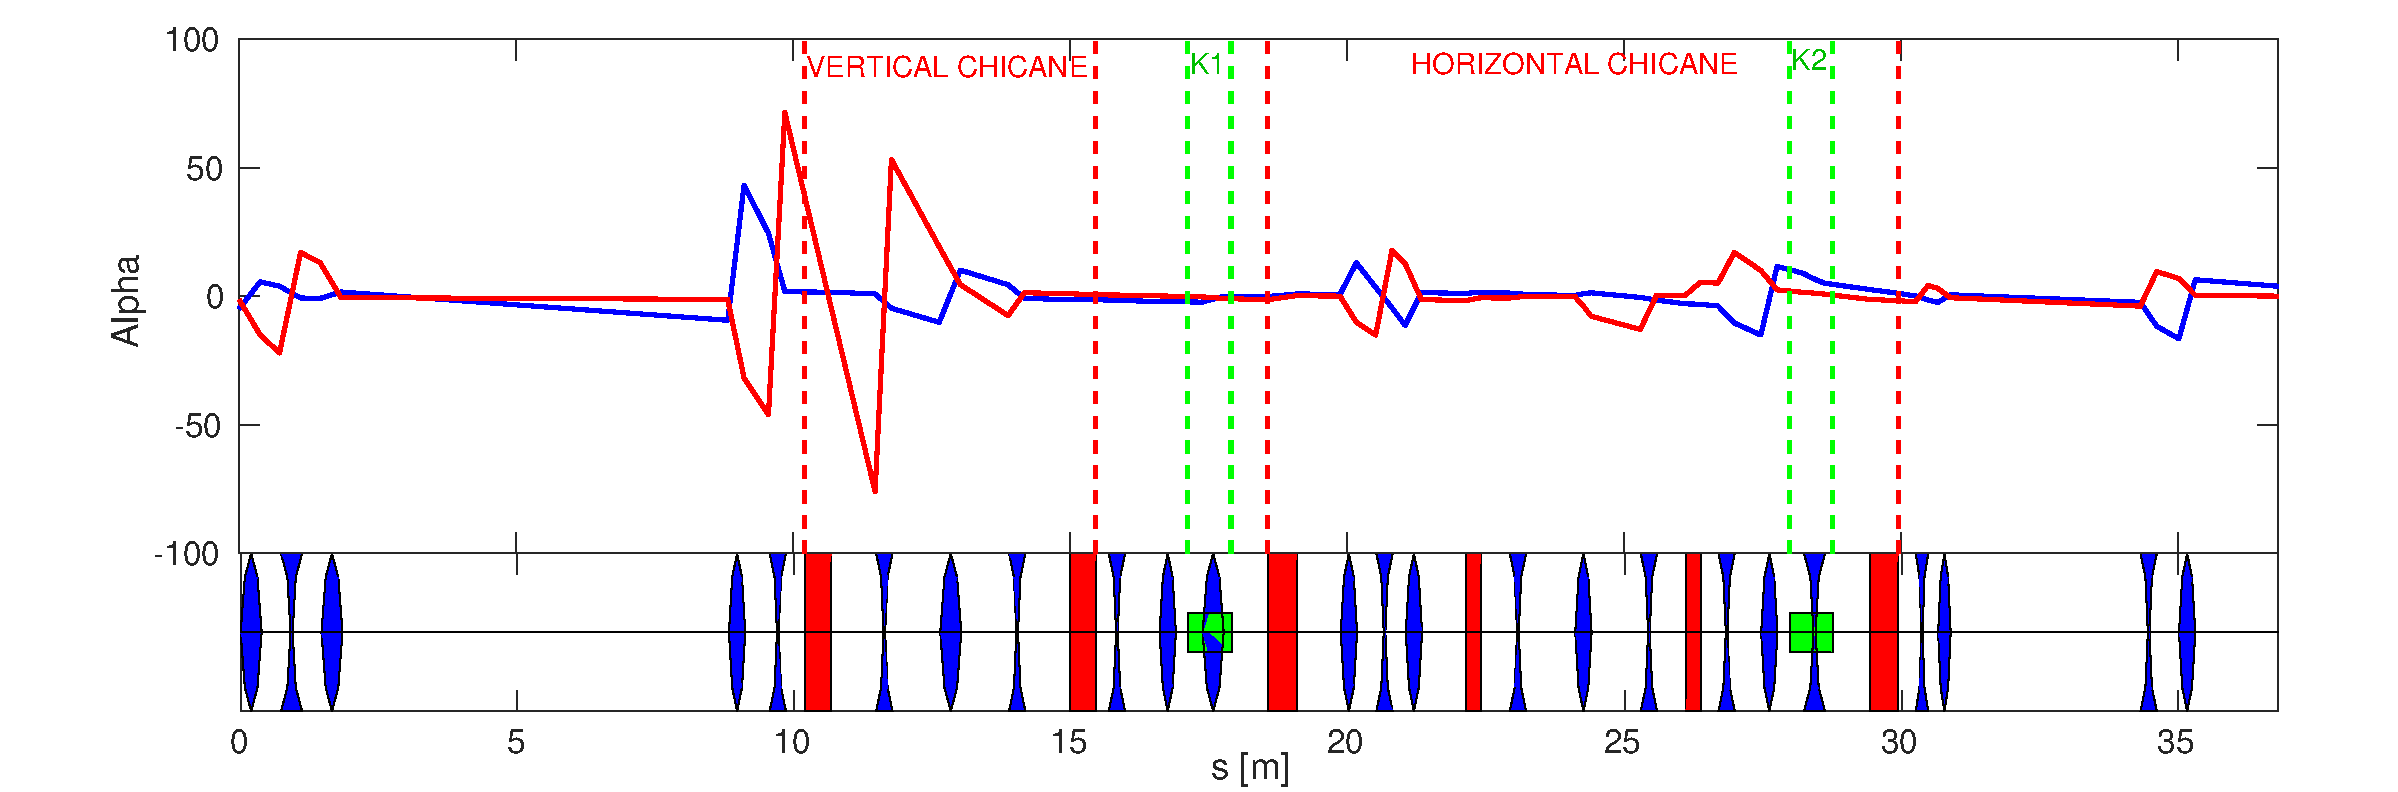
\includegraphics[width=0.85\hsize]{Figures/optics/pffOpticsAlpha}
  \caption{Horizontal and vertical alpha functions in the new TL2 optics.}
  \label{f:pffOpticsAlpha}
\end{figure}

\begin{figure}
  \centering
   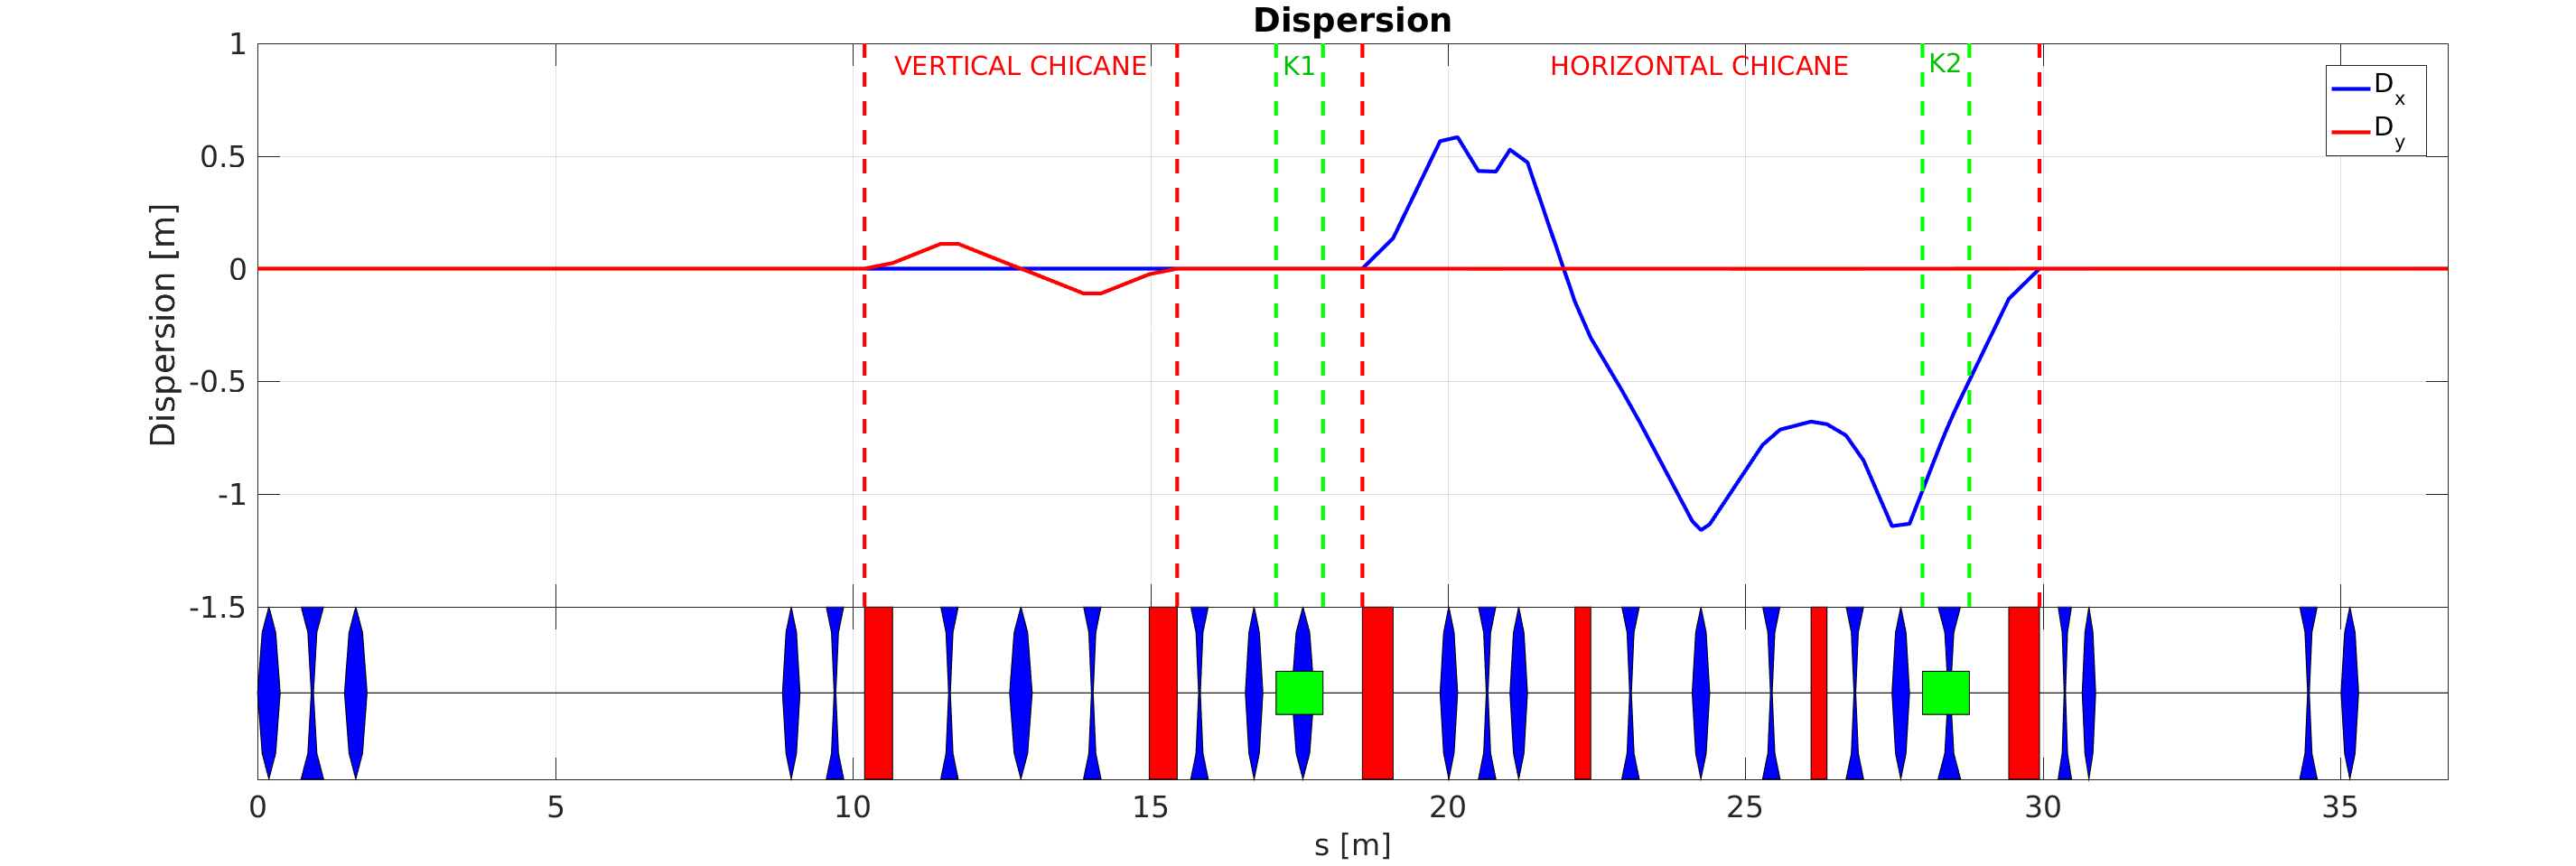
\includegraphics[width=0.85\hsize]{Figures/optics/pffOpticsDisp}
  \caption{Horizontal and vertical dispersion in the new TL2 optics.}
  \label{f:pffOpticsDisp}
  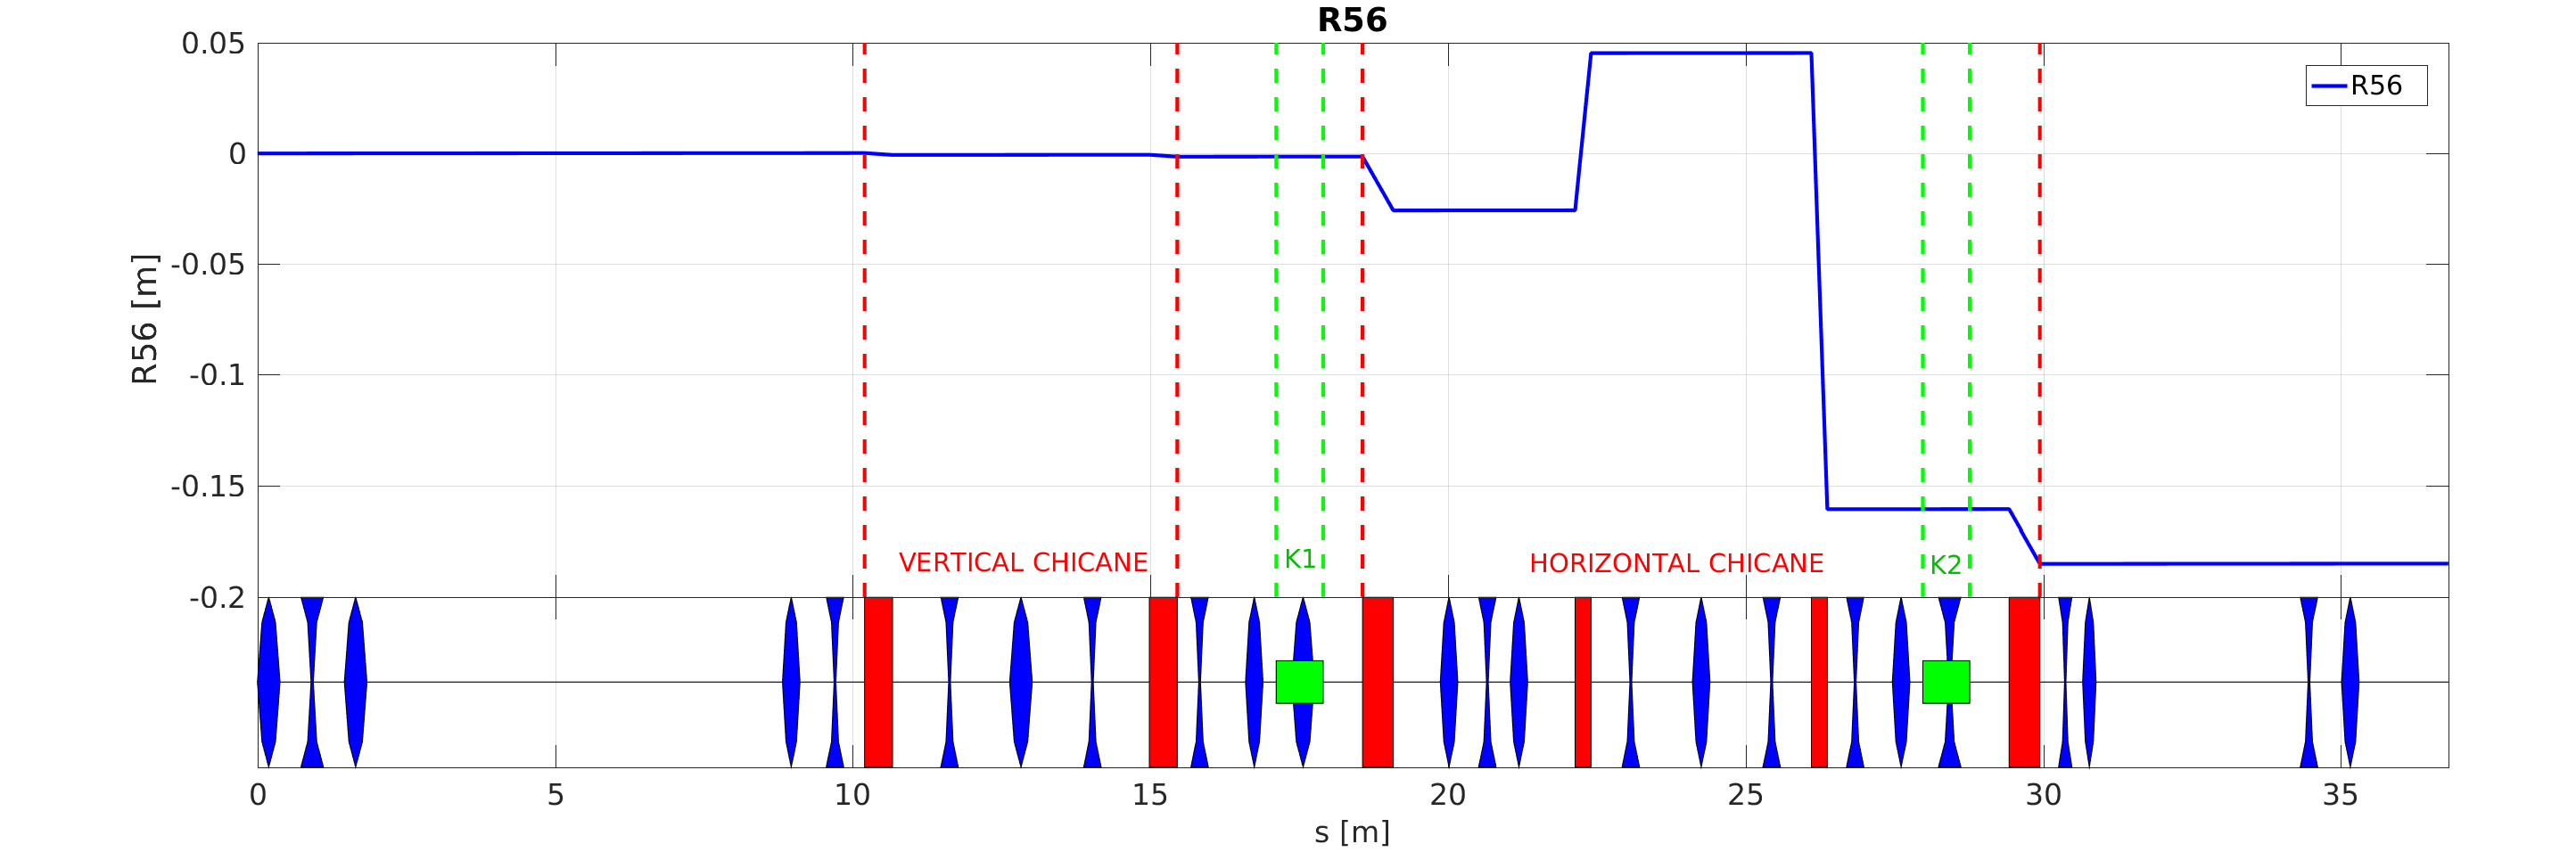
\includegraphics[width=0.85\hsize]{Figures/optics/pffOpticsR56}
  \caption{\(R_{56}\) in the new TL2 optics.}
  \label{f:pffOpticsR56}
\end{figure}

\begin{figure}
  \centering
  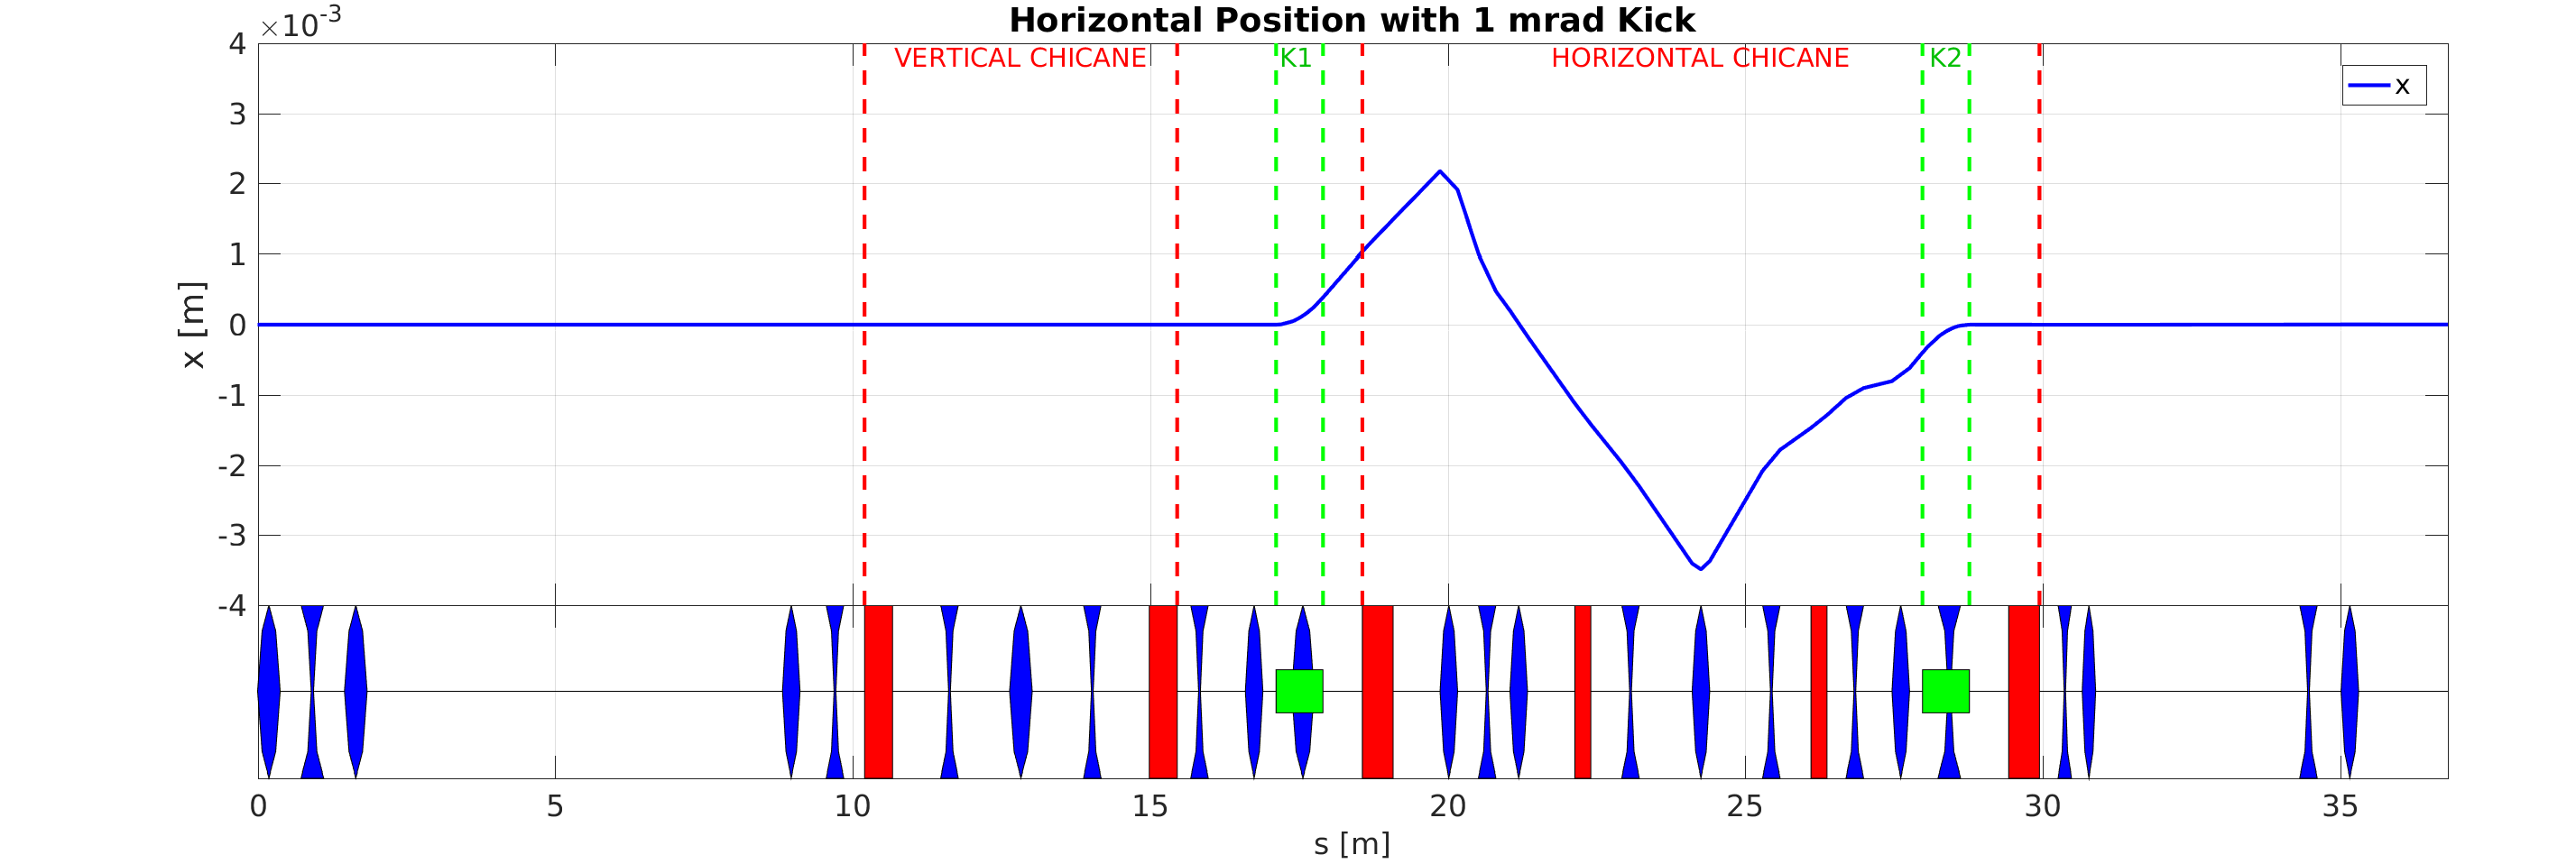
\includegraphics[width=0.85\hsize]{Figures/optics/pffOpticsX}
  \caption{Horizontal orbit in the TL2 chicane with a 1~mrad kick applied.}
  \label{f:pffOpticsX}
  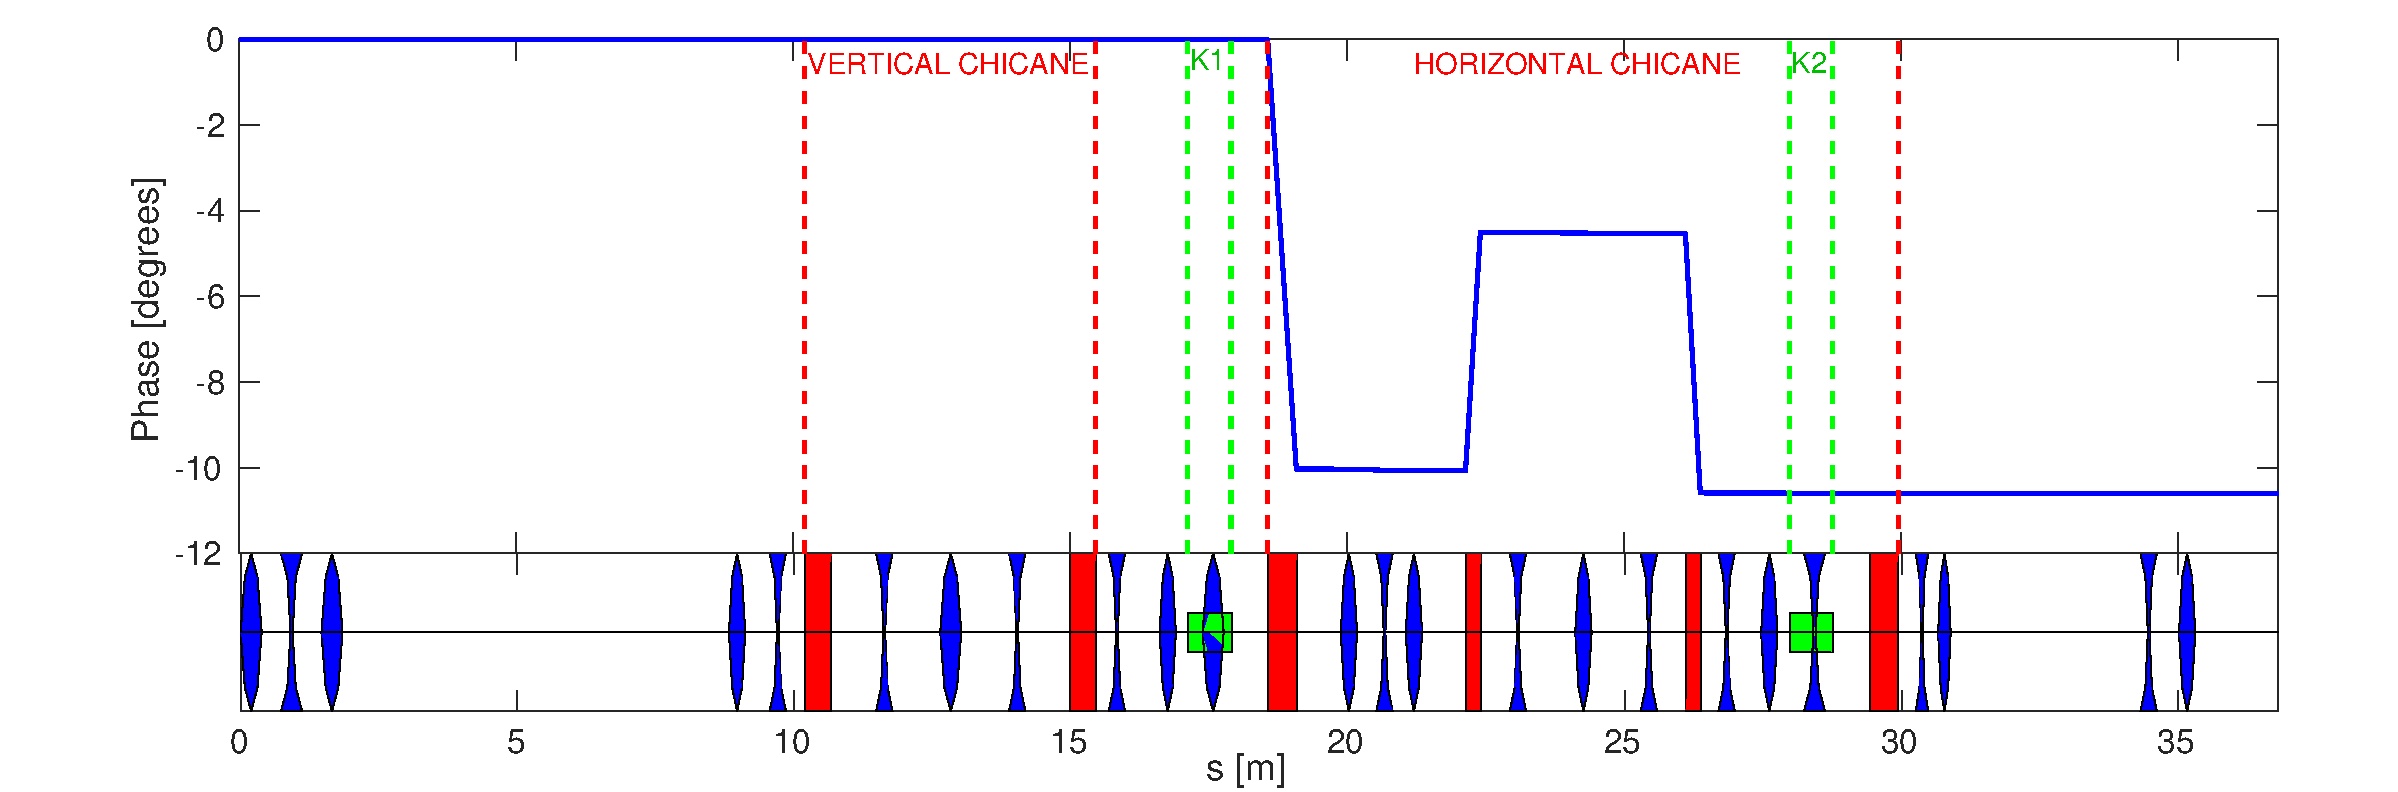
\includegraphics[width=0.85\hsize]{Figures/optics/pffOpticsPhase}
  \caption{Phase in the TL2 chicane with a 1~mrad kick applied.}
  \label{f:pffOpticsPhase}
\end{figure}
\end{landscape}